\chapter{Design of testing language}
\label{chap:Design}
This chapter introduces how the testing software (from now on tool) and the language introduced in Chapter \ref{chap:introduction} have been designed. The testing language specifies what a test does. A test is a series of verifications or modifications done on one or more HTTP messages (from now on messages) exchanged by the client and the service using the browser-based protocol. After the execution of a test, a check of the expected conditions has to be done, and the result has to be given to tell if the test has been successfully passed or not. The language will be defined based on all the possible actions that a security tester would need to do on the messages. 
One of the objectives was to think of a language that could specify the tests once and make it possible to test them over multiple web services. For example, a series of tests to verify the well-known vulnerabilities of a specific protocol could be defined and then used on any web service.

\section{Choosing a language standard}
A standard to follow while writing the tests had to be found; the first option was to define a formal language with its dedicated parser, this option was discarded, as it was challenging to implement and other already existing alternatives were available. The one that has been chosen is JSON (JavaScript Object Notation), which allows specifying the hierarchical structure of the tests using easy syntax writing. Also, its Object-oriented Notation is very useful, as tests and its components will be defined as Objects.

\section{Example: PKCE Downgrade Test}
\label{sec:pkce_downgrade}

I want to introduce the language with an example. Due to its complexity, having a concrete example before explaining all its components could be helpful to understand its function.
The scenario of this test is based on the presence of a web service hosted in a server (client), the victim, which is using a browser to connect to the client, the Authorization Server (AS) and the tester, that is doing a Man-In-The-Middle attack between the web service and the victim, and between the victim and the AS.

To understand this test, a brief introduction of \gls{PKCE} has to be done, \gls{PKCE} (Proof Key for Code Exchange) is an extension of the \gls{OAuth} protocol, as said in \cite{pkce_explanation}: \gls{PKCE}(pronounced pixie) extension describes a technique for public clients to mitigate the threat of having the authorization code intercepted. The technique involves the client first creating a secret and then using that secret again when exchanging the authorization code for an access token. This way if the code is intercepted, it will not be useful, since the token request relies on the initial secret. 
The \gls{PKCE} Downgrade test has as objective to test an \gls{OAuth} vulnerability were removing the parameter \texttt{code\_challenge} from the url of the authorization request message will be downgrading the authentication process in a way that \gls{PKCE} will not be used by the AS if the AS is vulnerable \cite{pkce_downgrade}. This will allow the attacker to steal the authorization code from the AS. The message sequence chart of the attack can be seen in Figure \ref{fig:pkce_downgrade}.

To test this, the browser will execute the victim's actions, doing a login on the client. The authorization request message has to be intercepted, the \texttt{code\_challenge} parameter has to be removed from it, and then the message has to be forwarded. The test is passed if the AS does not admit an exchange without PKCE; for instance, it can return an error page, which means that the AS is not vulnerable. Otherwise, if the AS would be vulnerable, the exchange would continue without any error pages or messages.
The complete test can be found in Attachment \ref{chap:PKCE_complete}

\begin{figure}[h]
    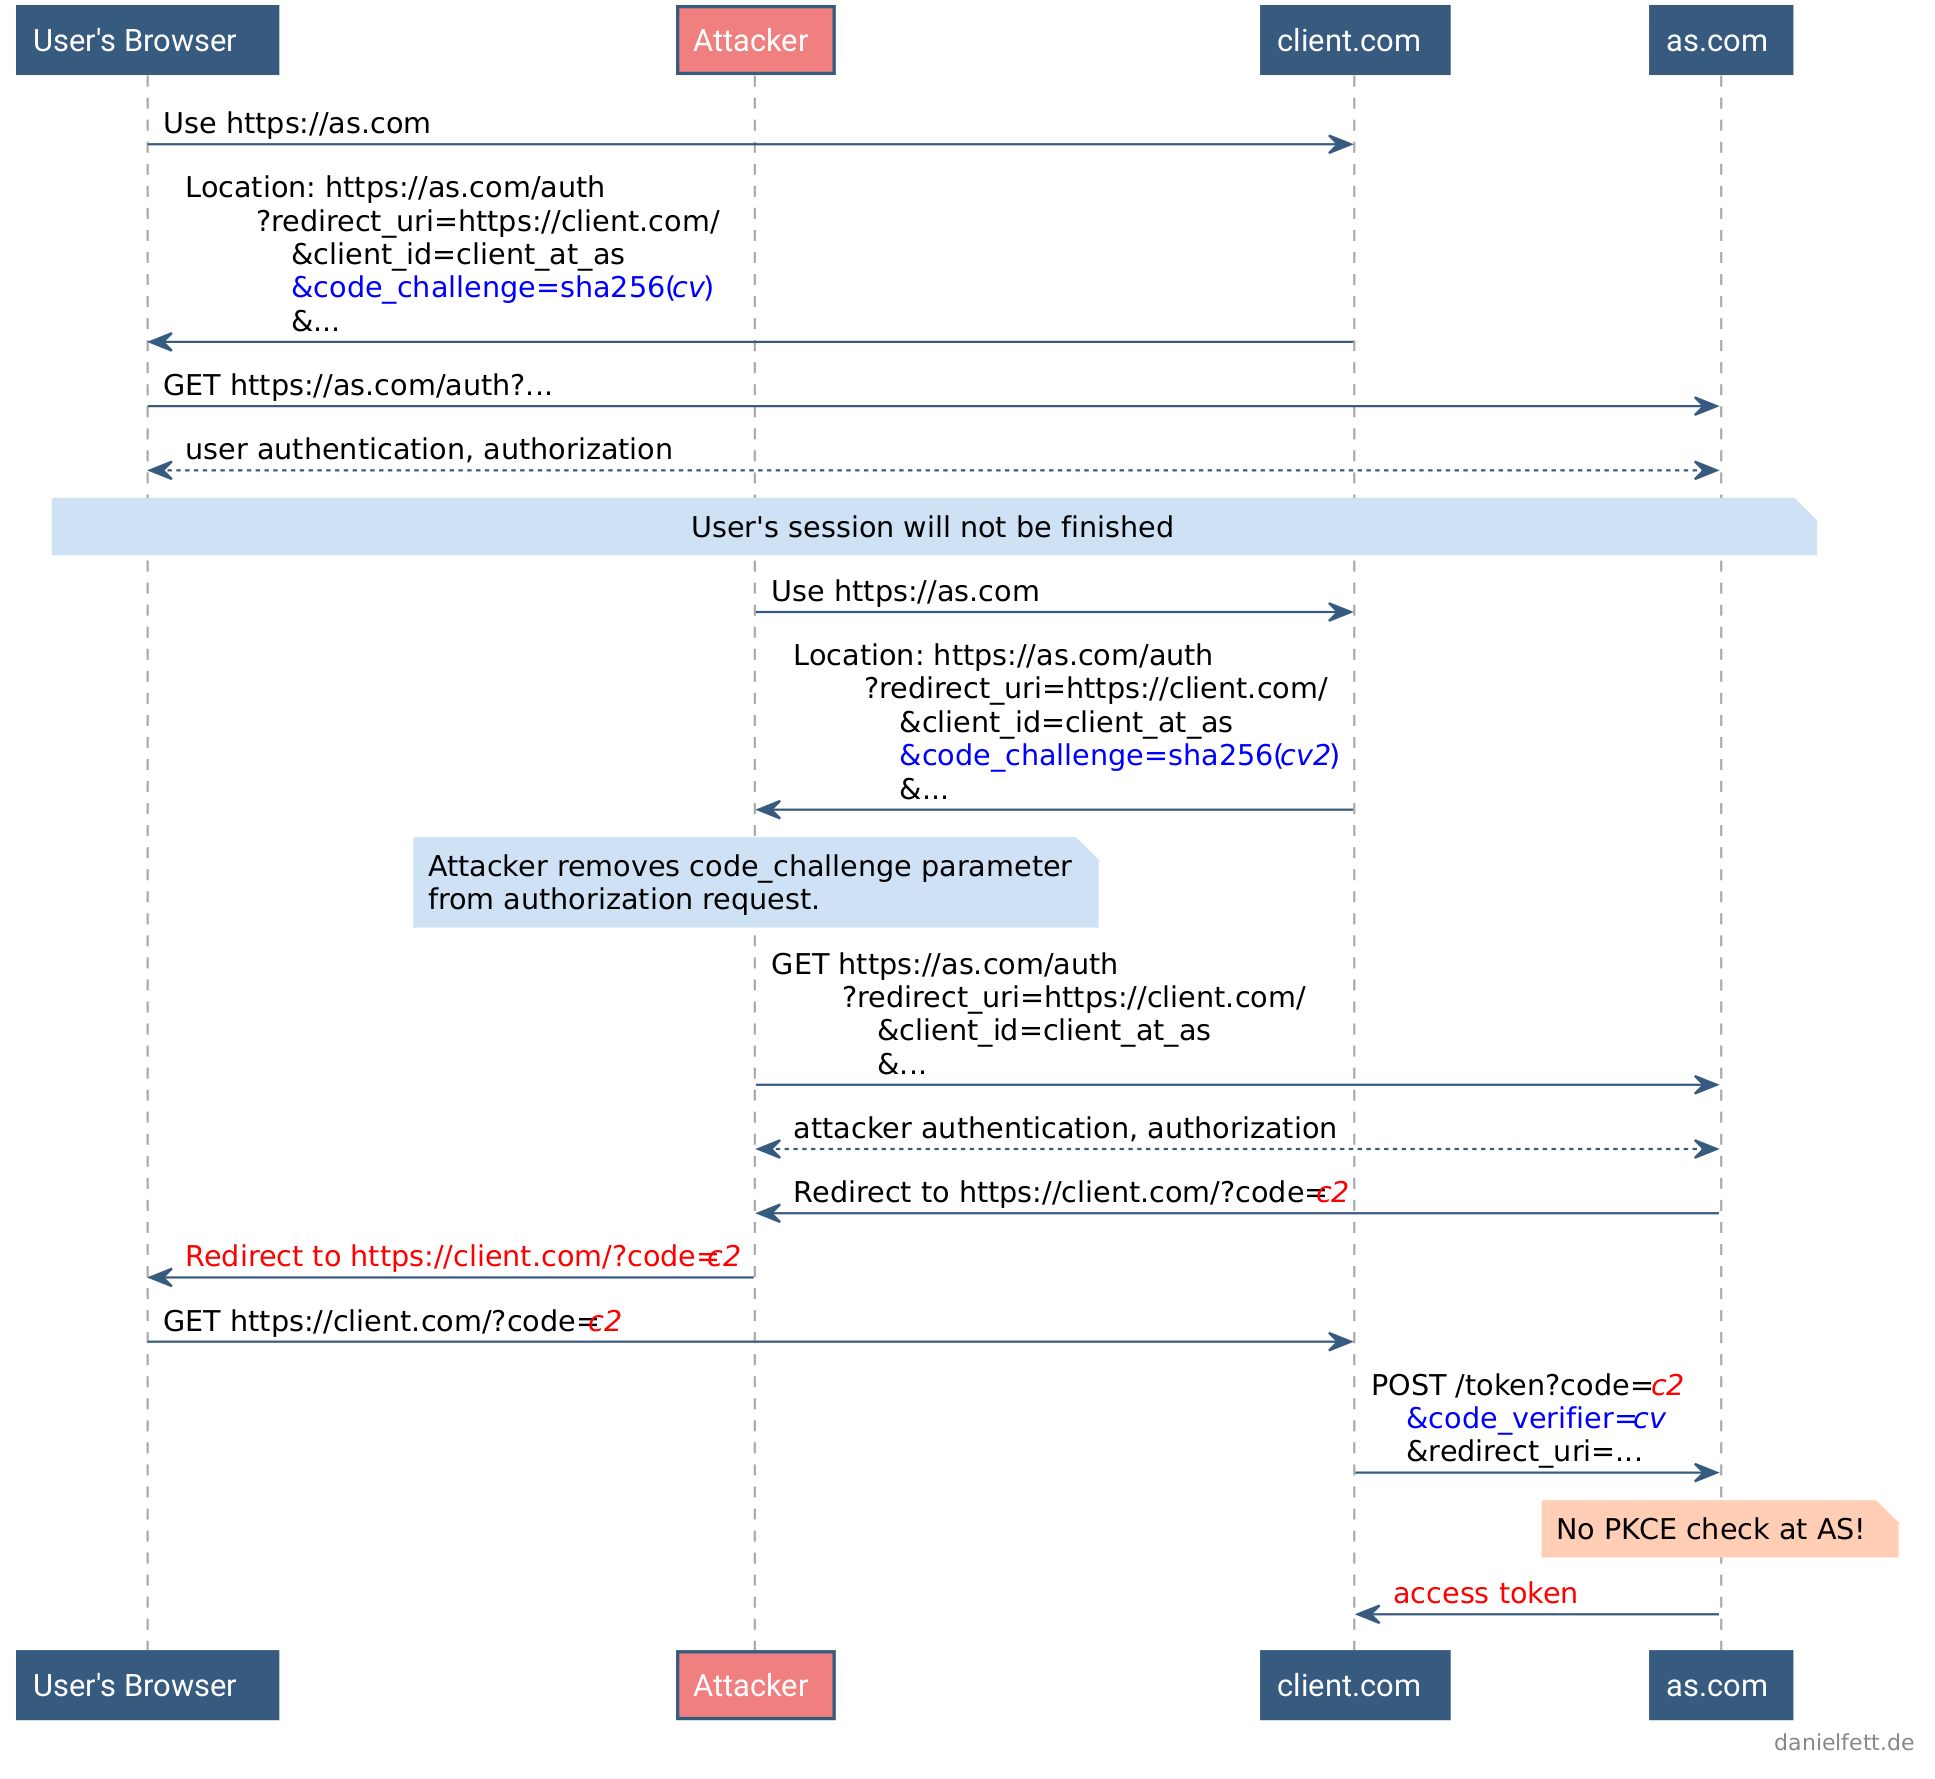
\includegraphics[width=\textwidth]{pkce_downgrade.png}
    \caption{PKCE Downgrade. Source: Daniel Fett \cite{pkce_msc_image}}
    \label{fig:pkce_downgrade}
\end{figure}

\section{Language structure}
Each part of the language is an Object, which is then written as a JSON Object in the language that contains a series of name/value couples. The hierarchical structure of the language can be seen in Figure \ref{fig:language_structure}. An example of a Test Suite Object containing other Objects can be seen in Figure \ref{fig:language_structure_2}. In this section, all the Objects composing the language will be discussed.

\begin{figure}
    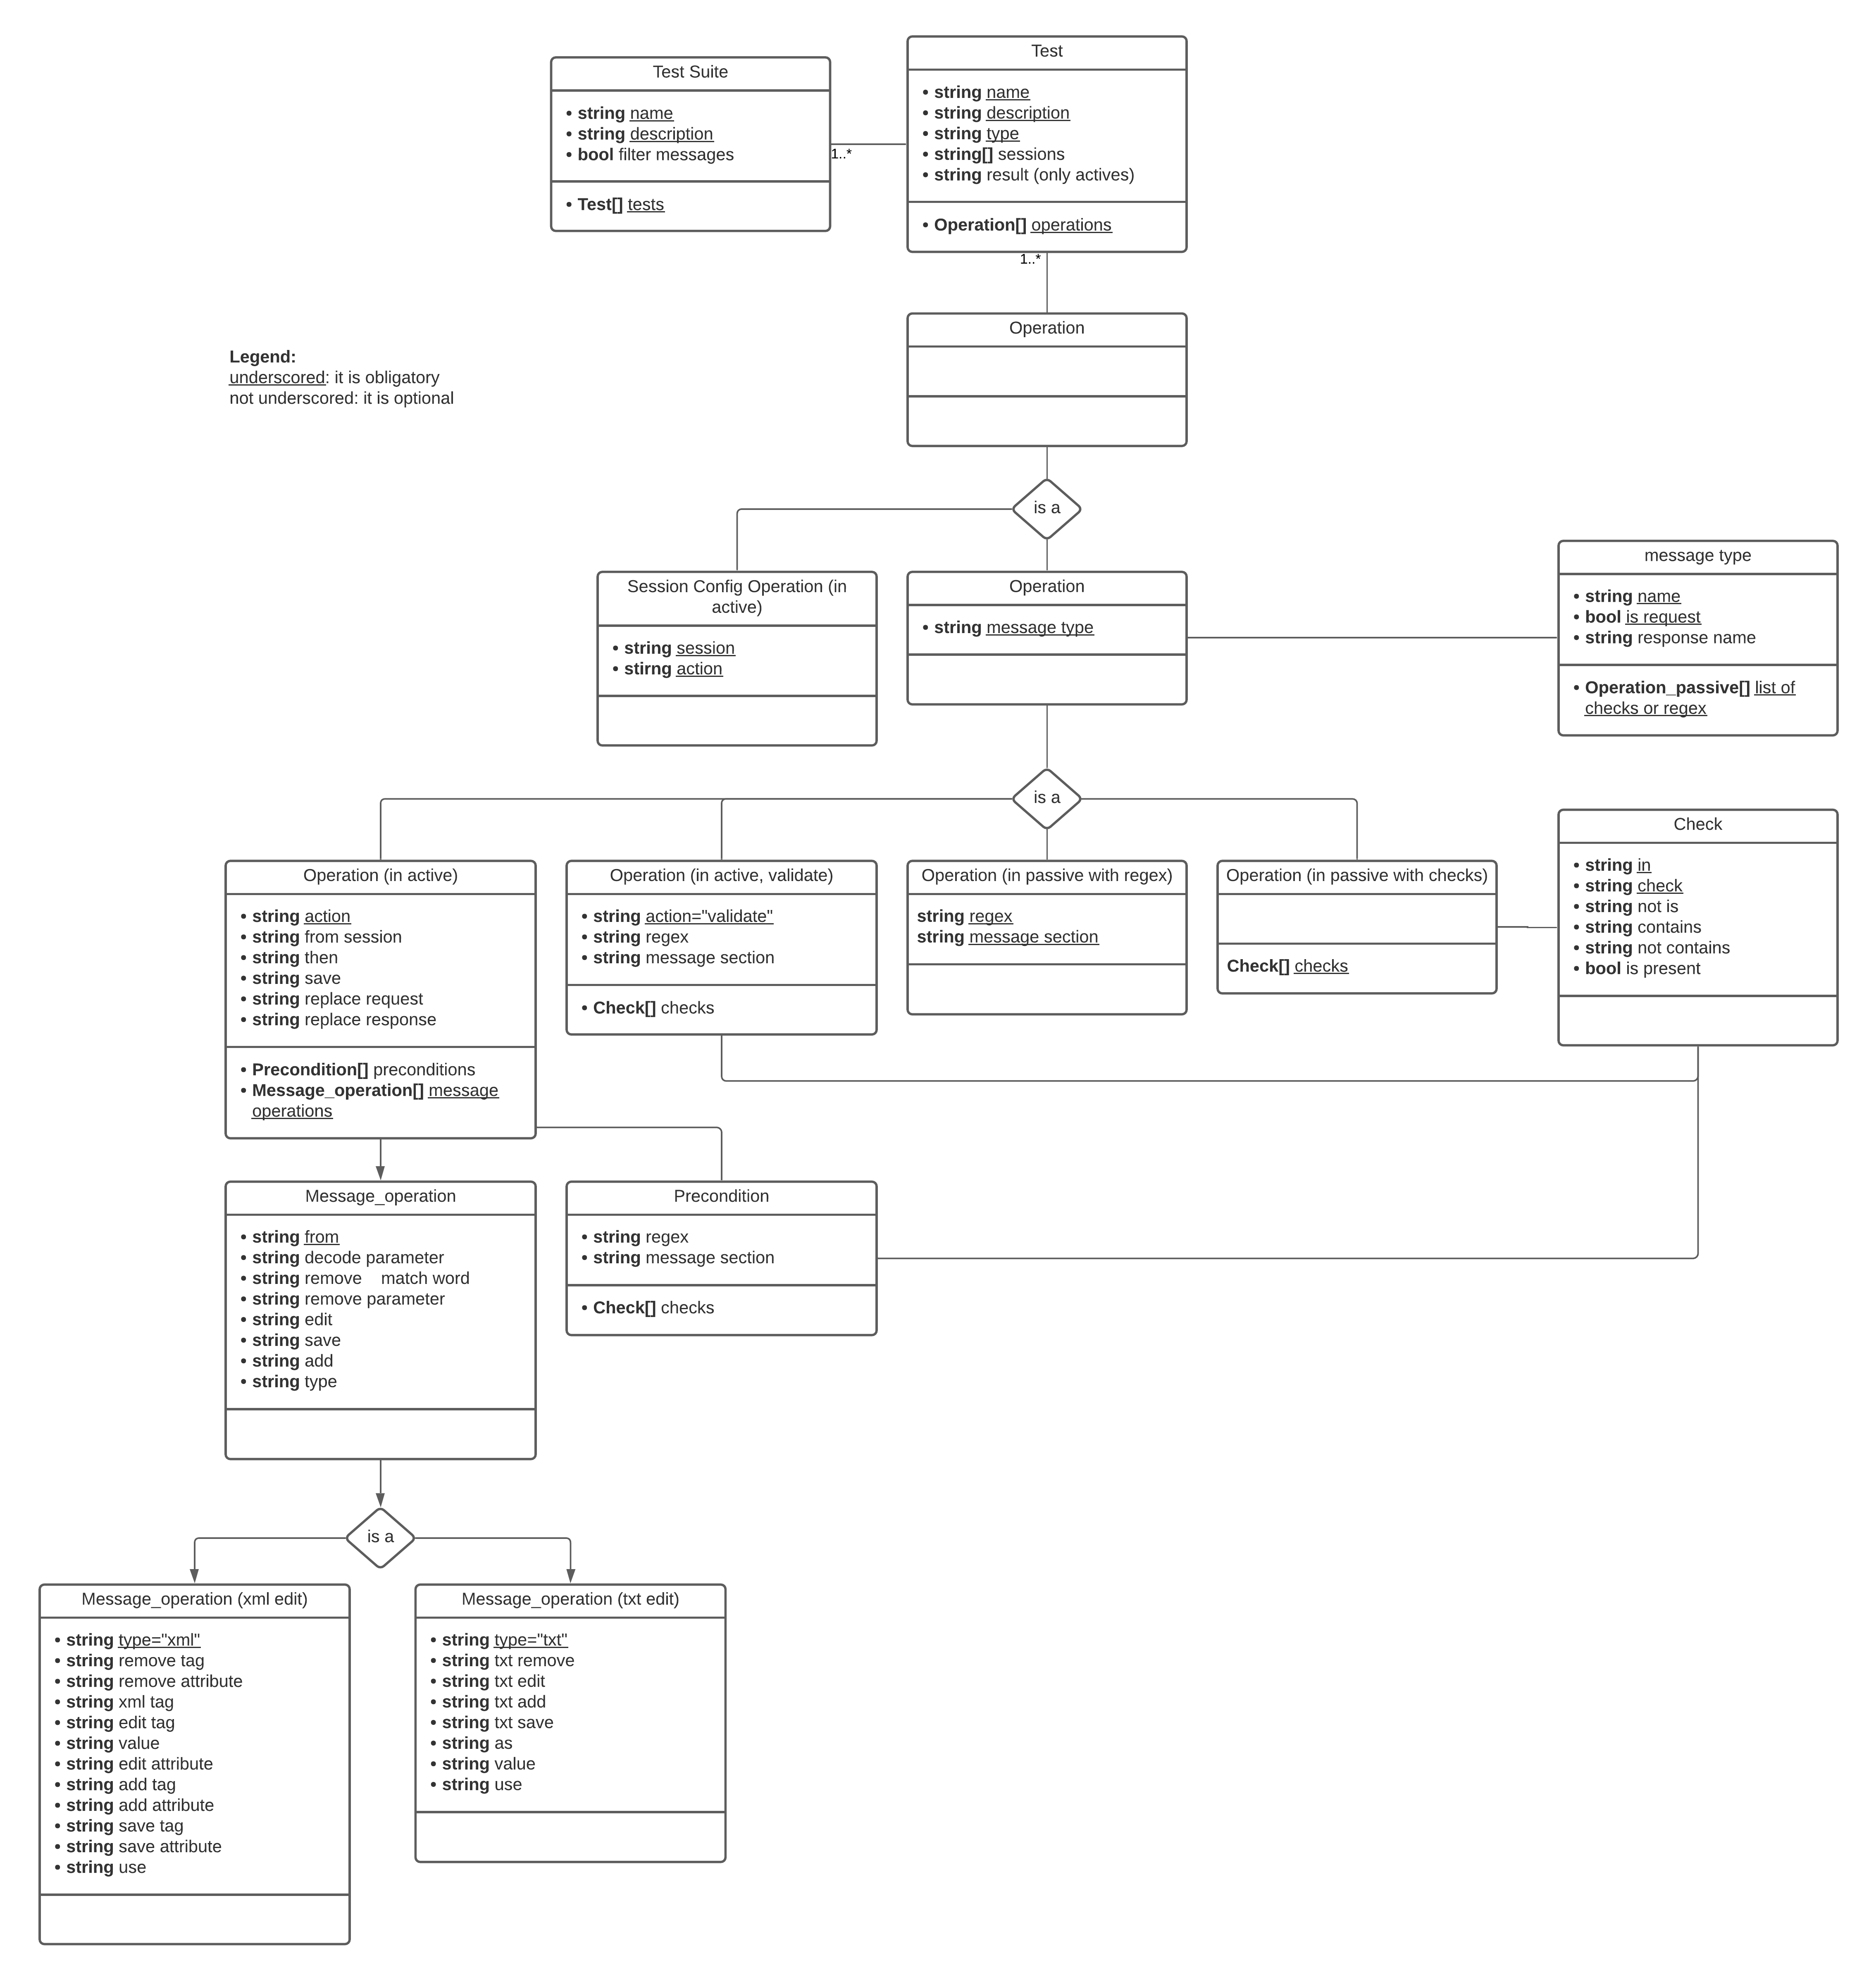
\includegraphics[width=\textwidth]{language_structure.png}
    \caption{Language structure}
    \label{fig:language_structure}
\end{figure}

\subsection{Test Suite}
The Test Suite is the main Object which contains all the other ones, it has these tags:

\begin{itemize}
    \item \textbf{name}, the name of the test suite
    \item \textbf{description}, the description of the test suite
    \item \textbf{tests}, which is a list containing the tests to be executed
\end{itemize}
To implement the \gls{PKCE} test example above, the Test Suite can be defined as shown in Listing \ref{lst:test_suite_definition}. The Test Suite Object is a JSON object having the tag \textbf{test suite}, with name and description, and a tag \textit{tests} which will contain a list of Test Objects.

\begin{lstlisting}[language=json, caption=Test Suite definition, label={lst:test_suite_definition}]
    {
        "test suite": {
            "name": "OAuth active tests",
            "description": "A test suite containing a OAuth test"
        },
        "tests": [
            {
                // A test
            }
        ]
    }
\end{lstlisting}

\subsection{Test}
Following the hierarchical order, the Test object is the one that actually defines a test. As said earlier, a test is contained in a Test Suite, and contains various tags to be defined:
\begin{itemize}
    \item \textbf{name}
    \item \textbf{description}
    \item \textbf{type}, it can be \textit{active} or \textit{passive}
    \item \textbf{sessions}, which is a list of the sessions which are needed in this test
    \item \textbf{result}, (only for actives) it defines the conditions over which the test is considered passed or not
    \item \textbf{operations}, a list of Operation objects which will be executed
\end{itemize}
A test can be defined either as active or passive depending on the type of actions it has to do on the intercepted messages. If a test does not need to manipulate the flow or the content of the messages, it is considered passive; otherwise, it is considered active.
The list of Operation Objects contained in a Test is executed iteratively one after the other, so only after an Operation is completed the next one starts.

Following the \gls{PKCE} example introduced in Section \ref{sec:pkce_downgrade}, an active Test is defined:

\begin{lstlisting}[language=json, caption=Active test definition, label={lst:active_test_definition}]
{
    "test": {
        "name": "PKCE Downgrade",
        "description": "Tries to remove code_challenge parameter",
        "type": "active",
        "sessions": [
            "s1"
        ],
        "operations": [
            // list of Operation Objects
        ],
        "result": "incorrect flow s1"
    }
}    
\end{lstlisting}

As can be seen in Listing \ref{lst:active_test_definition}, the test is specified, writing its type, which is active, as it has to edit a message removing a parameter from the url. Moreover, a session and a list of Operations to be executed are added. The result of the test is also specified.

\subsection{Operation}
\label{sec:operation}
\begin{wrapfigure}{r}{0.4\textwidth}
    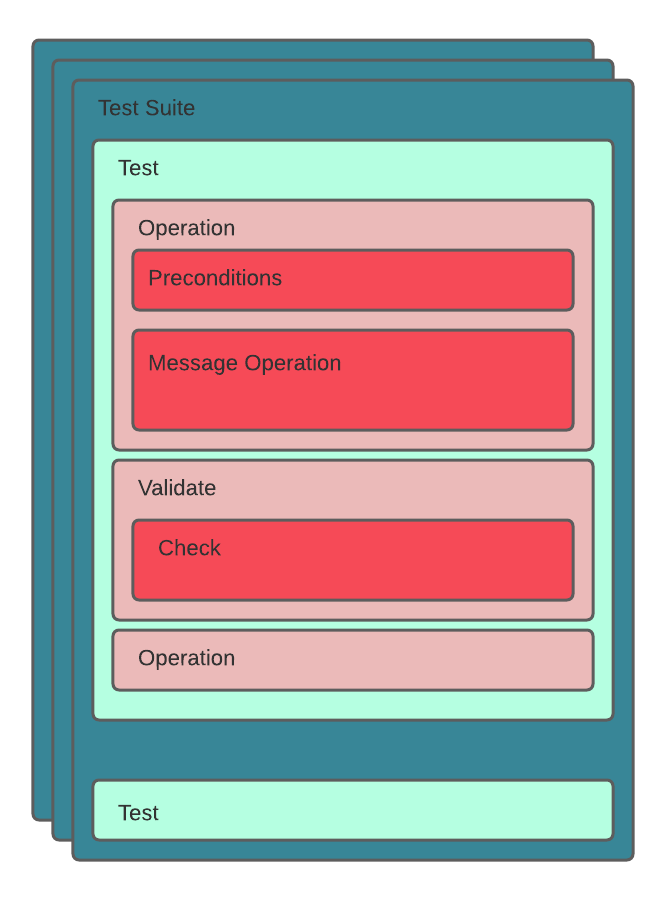
\includegraphics[width=0.9\linewidth]{language_structure_2.png}
    \caption{language structure}
    \label{fig:language_structure_2}
\end{wrapfigure}

The Operation Object defines the actions that a test has to do. As shown in the language structure in Figure \ref{fig:language_structure}, an operation could be either a \textbf{standard operation} or a \textbf{session config operation}, the latter is used to manage the sessions for the active tests (i.e. start, stop, pause them). Depending on the type of test in which an Operation is defined, the standard Operation becomes active or passive.
In both cases, an operation has to contain the \textbf{message type} which defines the type of message to be intercepted in that particular Operation (more info in the dedicated paragraph).
\\A \textbf{passive} operation has as objective to verify the presence (or absence) of some text or parameters in the intercepted message. To do this, it should contain one of the following options:
\begin{itemize}
    \item A list of \textbf{Check} Objects, which are then executed to check the presence (or absence) of some text or parameter
    \item A \textbf{regex} inspection, which executes an inspection considering the intercepted message as plain text and executing a regex over it; if the regex has a match, the Operation is considered passed, otherwise failed. Note that when a regex is used, it has to be also specified the \textbf{message section} over which to execute it (body, head, url)
\end{itemize}

If the Test Object where the operations are defined is an \textbf{active} test, also, if the intercepted messages need to be manipulated, an active Operation has to be defined. It is composed by:
\begin{itemize}
    \item \textbf{action}, the action it has to do (\textit{intercept}, \textit{validate})
    \item \textbf{from session}, from which session to expect the message to be intercepted
    \item \textbf{then}, the action to do after the receiving and manipulation of the message (forward or drop)
    \item \textbf{replace request (or response)}, specify a previously saved message in order to replace it to the intercepted one
    \item \textbf{preconditions}, a list of Precondition objects
    \item \textbf{message operations}, a list of Message Operation objects, which will do the actual manipulation of the intercepted message
\end{itemize}

If the action is set to \textit{validate}, the Operation is still active. However, it becomes like a passive Operation because its objective is just to verify that some messages meet some requirements. It will contain a regex or a list of checks to be done. The Validate Operation Object is part of the oracle, which is the component that decides whether the tests should be considered passed or not. More details will be discussed in the dedicated section.

In the \gls{PKCE} example seen in Section \ref{sec:pkce_downgrade}, an Operation Object for an active test is specified. This Operation has to intercept the \textit{authorization request} message from session \textit{s1}. It has to check some Preconditions over it and then do some Message Operations. In the end, the message is forwarded to its original destination.

\begin{lstlisting}[language=json, caption=Operation definition]
{
    "action": "intercept",
    "from session": "s1",
    "then": "forward",
    "message type": "authorization request",
    "preconditions": [
        // Precondition list
    ],
    "message operations": [
        // Message Operation list
    ]
}
\end{lstlisting}

\subsection{Message section}
The message section specifies in what part of the message to execute the given action.
According to \cite{http} the parts that compose an HTTP message are:
\begin{itemize}
    \item \textbf{url}, a start line describing the message
    \item \textbf{head}, a block of headers containing attributes
    \item \textbf{body}, an optional body containing data
\end{itemize}

\subsection{Check Object}
The Check Object is used in Operations Objects and in other Objects to verify that, in a message, some circumstances are satisfied. For instance, it can be used to check that a specific parameter in the url of a message should be equal to a specific string.
The Check Object is defined by:
\begin{itemize}
    \item \textbf{in}, where to search the given parameter. The possible value is \textit{head}, \textit{body} or \textit{url}
    \item \textbf{check param}, specifies the parameter name to be searched
\end{itemize}
Also, the actual checks on the parameter value have to be defined: (if none of these are defined, the Check will only check if the given parameter is present or not in the given section)
\begin{itemize}
    \item \textbf{is}, checks that the parameter value is exactly what is passed to this tag
    \item \textbf{not is}, checks that the parameter value is not what is passed to this tag
    \item \textbf{contains}, checks that the parameter value contains what is passed to this tag 
    \item \textbf{not contains}, checks that the parameter value does not contain what is passed to this tag 
    \item \textbf{is present}, used to explicitly tell to just check the presence of the parameter, it accepts true or false, depending on if, respectively, the presence or the absence of the parameter has to be checked.
\end{itemize}

Note that by how the logic of the language has been thought, to consider a test passed, all the check Objects has to be evaluated to true. For instance, if a parameter should not be present in a given message, the Check has to verify that the parameter is \textbf{not} present. If a Check is evaluated to false, the test will fail.

\subsection{Precondition and Validate Objects}
In active tests, Check Objects will not work as in passive tests, there is another way of using them: using them in a Precondition, which is a list of the Check Objects, or by using the validate option in an Operation Object, which will make possible to use Checks to validate a given message. This difference of Check Objects between active and passive tests has been made to allow the Oracle to work, differentiating between a precondition and a validation. This way, Validate Objects can be used to define the oracle, and Precondition Objects can be used to impose the criteria to allow the execution of the test.
\paragraph{Precondition Object}
Preconditions are used in an Operation of an active test to check that the intercepted message complies with specific criteria fixed by the tester before executing the Message Operations. If the Check objects in the precondition are evaluated to false, the test is considered unsupported, not failed. More precisely, the preconditions will be a list of Check Objects. This can be useful in case it is not known if a given test is compatible with a given web service. For example, if the service does not use some protocol, this can be assured by using preconditions checking for the presence of common parameters of the protocol. Preconditions can also be a regex.
\paragraph{Validate Object}
In an Operation Object, the only way to use Check objects is by setting the \textbf{action} tag to \textit{validate}. This will transform the Operation into a Validate Operation. The Oracle will use this Validate Operation to decide whether the test should be considered passed or not. Validate Operation has to be used when a given part of a message should be in a specific way. If it is not, the test result will be considered failed.
In order to do this, the Validate Operation with a list of checks or a regex (exactly like in passive tests) can be used.

\subsection{Save}
A message or a string can be saved by the use of the tag \textbf{save}. This can be used both in an Operation to save an entire message or in a Message Operation to save the value of a found parameter. So a variable can be a message-type variable, containing an entire saved message or a string-type containing a string.
There are two ways of using the value of a variable which depends on its type:
\begin{itemize}
    \item Using a \textbf{message-type} variable: it can be used in an Operation with the tag \textbf{action} set to intercept. There is the possibility of using \textbf{replace request} (or \textbf{replace response}) tag giving the name of the variable. This will replace the intercepted message's request (or response) with the message saved in the variable.
    \item Using a \textbf{string-type} variable: can be used in Message Operations, where a parameter has to be edited, writing \textbf{use} tag specifying the name of the variable to use. This will use the value in that variable in the way specified by the other tags (i.e., tags \textbf{edit} or \textbf{add})
\end{itemize}

\subsection{Message Operation}
The Message Operation is the Object that actually does the manipulations on the intercepted messages. It is composed by these tags:
\begin{itemize}
    \item \textbf{from}, the message section to work on
    \item \textbf{decode parameter} (optional) it indicates which parameter's value or string to be decoded before it can be processed
    \item \textbf{encodings} (optional) the list of encodings to be applied to the parameter or text to be decoded. The supported encodings are base64, deflate, url
    \item \textbf{remove match word} (optional), it accepts a regex, everything matched by that regex in the specified message section is removed
    \item \textbf{remove parameter}, it accepts a parameter name, it removes both the name and the value of that parameter from the specified section
    \item \textbf{edit}, it accepts a parameter name, and edits its value with the new value specified with \textbf{in} tag
    \item \textbf{save}, (optional) it accepts a parameter name, the value of that parameter is saved in a variable, it is necessary to specify the name of the variable using \textbf{as} tag
    \item \textbf{add}, (optional) it accepts a parameter name, it appends to the parameter value the string passed with \textbf{this} tag
    \item \textbf{type} (optional) specify how the decoded parameter should be interpreted (txt or xml)
\end{itemize}

In a Message Operation, there is the possibility to specify a parameter or some text to be decoded before manipulation. To do that, specify with \textbf{decode parameter} the parameter to be decoded and with \textbf{encodings} the encodings necessary to decode the parameter. The order of definition of the \textbf{encodings} will be followed during decoding. The parameter (or text) decoded will be encoded again automatically at the end of the Message operation before forwarding it.
The decoded parameter can be manipulated using the \textbf{type} tag. There is the possibility to interpret the decoded parameter by two means: 

\paragraph{Type txt}
Associated with this interpretation, it is possible to use a list of actions over the plain text:
\begin{itemize}
    \item txt remove: removes the matched string from the decoded parameter
    \item txt edit: edits the matched string with a custom string (specified with the \textbf{value} tag)
    \item txt add: after the matched string adds a string specified with the \textbf{value} tag
    \item txt save: saves the matched string in a variable with the name specified in the \textbf{as} tag
\end{itemize}
All the previous tags accept a regex, and anything that regex matches will be edited, added, or saved based on the specified tag.

\paragraph{Type xml}
Another possibility is to interpret the decoded text as XML. To do this, the type tag has to be set to \textit{xml}.
This way the various possible operations to be done on the decoded xml are:
\begin{itemize}
    \item \textbf{remove tag}, removes the specified tag
    \item \textbf{remove attribute}, removes the specified attribute associated with the xml tag specified using the \textbf{xml tag}
    \item \textbf{edit tag}, edits the specified tag with the value contained in \textbf{value} tag 
    \item \textbf{edit attribute}, edits the specified attribute associated with the xml tag specified using the \textbf{xml tag}
    \item \textbf{add tag}, adds the specified tag, having the value specified with tag \textbf{value}, and also the name of the parent xml node to add the new node to, has to be specified using the \textbf{xml tag}
    \item \textbf{add attribute}, adds the specified attribute associated with the xml tag specified using the \textbf{xml tag}
    \item \textbf{save tag}, saves the specified tag value
    \item \textbf{save attribute}, saves the specified attribute value associated with the xml tag specified using the \textbf{xml tag}
\end{itemize}

In the \gls{PKCE} example found in Section \ref{sec:pkce_downgrade}, a simple Message Operation is present, which has to remove the parameter \texttt{code\_challenge} from the url of the message, so the resulting Message Operation will be:
\begin{lstlisting}[language=json, caption=Message Operation definition]
{
    "from": "url",
    "remove parameter": "code_challenge"
}
\end{lstlisting}

\paragraph{Note for body section in message operations}
If the \textit{body} section is chosen, the meaning of the following tags becomes different:
\begin{itemize}
    \item \textbf{remove parameter} will work like \textbf{remove match word}, in a way that the value of the tag is treated as a regex which will be matching against the entire body section, having all the matches removed from it
    \item \textbf{edit} is treated as a regex, substituting everything that matches that regex with the text specified by the \textbf{in} tag
    \item \textbf{save} is treated as a regex, saving what will be matched by the regex, the name of the variable in which the value will be saved is specified with the \textbf{as} tag
    \item \textbf{add} is associated with a regex. It will add at the end of the matched text the value specified by \textbf{this} tag
\end{itemize}

This also changes for the \textbf{decode parameter} tag, in a way that if the message section is 'body', the \textbf{decode param} will accept a regex, and everything matched by that regex will be considered to be decoded. \\ An example of a regex to match a parameter in the body could be ``\verb|(?<=parameter_name=)[^$\n& ]*|" that will search for the text ``parameter\_name", taking everything after the ``=" until end of line or ``\&" or whitespace is found.

This difference in the tag meaning is due to the difficulty of identifying parameters in the body section in contrast to the head section. While the head section is based on the HTTP standard, having all parameters defined in a clear and well-defined way like ``Name: value" the body section could contain any type of content. To manage this variety of contents, the decision to use regex instead of parameter names for the body section has been chosen.

\subsection{Message Type definition}
The message type definition is needed to define some types of messages that will be later used in the language to intercept them.
The message type definition is not part of the language, but it is stored in a file in the \Gls{burp} folder. The definition of the type of messages uses the same Objects as the language.
A Message Type Object is defined using these tags:
\begin{itemize}
    \item \textbf{name}, the name that will be used in the language to refer to this message type
    \item \textbf{is request}, if set to true if the searched message is a request, false otherwise
    \item \textbf{response name}, if the searched message is a request message, this tag can be used to associate a name to the response of that message. This is useful when only the request message can be identified, allowing to intercept the correlated response message.
    \item \textbf{checks}, a list of Check objects used to identify the message. If evaluated to true, the message is considered found
\end{itemize}

Following the example from Section \ref{sec:pkce_downgrade} the definition of the \textit{authorization request} message used in the test, and can be found in the Listing \ref{lst:msg_def}.

\begin{lstlisting}[language=json, caption=Message Types definition, label={lst:msg_def}]
{
    "message_types": [
        {
            "name": "authorization request",
            "is request": true,
            "response name": "authorization response",
            "checks": [
                {
                    "in": "url",
                    "check param": "response_type",
                    "is present": "true"
                }
            ]
        },
    ]
}
\end{lstlisting}

When used, this message type will search for the parameter \texttt{response\_type} in the url of every request message. When a match is found, the Operation in which this Message Type is used will be executed.

\section{The oracle}
The set of all parts of the language that decide the result of the tests is called Oracle,
which decides whether a test should be considered passed or failed (or not applicable). I decided to build the oracle in a way that it can be almost fully customized by the user. 
The oracle is based on three main components:
\begin{itemize}
    \item Evaluation of the complete (or incomplete) execution of the \gls{session track} 
    \item Evaluation of the Precondition objects
    \item Evaluation of the Validate objects
\end{itemize}
If all the above conditions are met, the test is considered passed. Otherwise, it is considered failed (or not applicable).
The oracle can be built, for example, by using Validate objects to verify that some intercepted messages satisfy some conditions like having a particular parameter or string in them.

To build the oracle for the \gls{PKCE} example mentioned in Section \ref{sec:pkce_downgrade}, both the result of the test and the precondition has been used, specifically, the precondition part is shown in Listing \ref{lst:precondtion}
\begin{lstlisting}[language=json, caption=Precondition definition, label={lst:precondtion}]
"preconditions": [
    {
        "in": "url",
        "check param": "code_challenge",
        "is present": true
    }
],
\end{lstlisting}
This precondition is used to consider the test ``not applicable" if the parameter \texttt{code\_challenge} is not found in the authorization request message. This means it is not possible to execute the given test over the actual intercepted message if the preconditions are not satisfied.

The \textbf{result} tag of the Test in the \gls{PKCE} example in Section \ref{sec:pkce_downgrade} is set to:
\begin{lstlisting}[language=json]
"result": "incorrect flow s1"
\end{lstlisting}
This means that the oracle will consider the test passed, if and only if the execution of the \gls{session track} of the session named \textit{s1} will be incorrect. The execution is considered incorrect when the execution of the \gls{session track} fails. This can be, for instance, because an unexpected page is displayed or an element that should be clicked is not present on the page. In the case of the PKCE example in Section \ref{sec:pkce_downgrade} the test is passed if the removal of the parameter \texttt{code\_challenge} is not admitted by the AS; usually, if this is the case, an error page will be displayed.

\section{Sessions}
A session is a browser executing a \gls{session track}, a \gls{session track} is a list of user actions that the browser will simulate automatically during execution of the Tests. There is the possibility of defining and using more than one session so that, e.g., reply tests can be executed. Different sessions can have different session tracks.

As said in Section \ref{sec:operation}, a \textbf{from session} tag can be specified in the Operation, this will specify in which session to search the message. To define the \gls{session track} the idea used in \cite{claudio_grisenti,stefano_facchini}, has been used, adding some options like \textbf{wait} and \textbf{clear cookies} functionalities.
The syntax of the \gls{session track} is based on the plain text export of Katalon Recorder \cite{katalon_recorder_syntax}. 
An example of a \gls{session track} that does the login at Unitn website is this:

\begin{lstlisting}[caption=Session track Unitn login]
    open | https://www.google.com/ |
    click | id=L2AGLb |
    click | link=Accedi |
    click | id=identifierId |
    type | id=identifierId | matteo.bitussi@studenti.unitn.it
    click | id=identifierNext |
    click | id=clid |
    type | id=clid | matteo.bitussi@unitn.it
    click | id=inputPassword |
    type | id=inputPassword | password
    click | id=btnAccedi |
    click | link=Gmail |
\end{lstlisting}

This \gls{session track} will do the login on the Unitn website using some credentials and password. The supported actions are:
\begin{itemize}
    \item \textbf{open $|$ url $|$}, to open an url
    \item \textbf{click $|$ id=, link=, xpath= $|$}, to click on a http object with the given id, link or xpath
    \item \textbf{type $|$ id= $|$ text}, to write on a given http element the given text
    \item \textbf{wait $|$ milliseconds}, to make the execution of the session wait for a given time 
    \item \textbf{clear cookies $|$}, to make the browser of the session clear all the cookies in it
\end{itemize}



